\chapter{Results}\label{chap:res_and_lit}


The tests ran over all the (counter) satisfiable \ac{epr} problems in TPTP v6.1.0, and they were 267 problem. We had a bash script running the transformations in the beginning then the normal prover then the model extraction part. Also it prints the time taken by each step. Moreover, time limit of 3 minutes was given to the 2nd step which is the normal prover itself. Only 107 of the problems were able to terminate within the time limit. 


The tests were done in a server having the following specification:
\begin{itemize}
	\item 8 GB RAM
	\item 8 CPUs
\end{itemize}


The below table ~\ref{table:sat_epr_results} is the results of running the script on all the 267 problem:

%\begin{table}[H]
%	\centering
	\begin{longtable}{||c | c | c | c | c | c||} 
 		\toprule
		Problem & rating & transformations t. & terminated
		& saturation t. & model extraction t. \\ %[0.5ex] 
		\midrule
GRP123-1.005.p & 0.17 & 0.003s & no & -- & -- \\
GRP123-2.005.p & 0.17 & 0.003s & no & -- & -- \\
GRP123-3.004.p & 0.17 & 0.008s & yes & 0.349s & 0.014s \\
GRP123-4.004.p & 0.17 & 0.004s & yes & 2.023s & 0.050s \\
GRP123-6.005.p & 0.17 & 0.004s & no & -- & -- \\
GRP123-7.005.p & 0.33 & 0.003s & no & -- & -- \\
GRP123-8.004.p & 0.17 & 0.003s & yes & 0.871s & 0.029s \\
GRP123-9.004.p & 0.17 & 0.003s & yes & 0.506s & 0.031s \\
GRP124-1.005.p & 0.17 & 0.006s & no & -- & -- \\
GRP124-2.005.p & 0.17 & 0.003s & no & -- & -- \\
GRP124-3.005.p & 0.17 & 0.004s & no & -- & -- \\
GRP124-4.005.p & 0.17 & 0.003s & no & -- & -- \\
GRP124-6.005.p & 0.17 & 0.007s & no & -- & -- \\
GRP124-7.005.p & 0.33 & 0.003s & no & -- & -- \\
GRP124-8.005.p & 0.33 & 0.003s & no & -- & -- \\
GRP124-9.005.p & 0.33 & 0.004s & no & -- & -- \\
GRP125-1.004.p & 0.17 & 0.003s & yes & 0.424s & 0.014s \\
GRP125-2.004.p & 0.17 & 0.003s & yes & 0.081s & 0.004s \\
GRP125-3.004.p & 0.17 & 0.005s & yes & 0.486s & 0.007s \\
GRP125-4.004.p & 0.17 & 0.002s & yes & 2.288s & 0.030s \\
GRP126-1.005.p & 0.17 & 0.004s & no & -- & -- \\
GRP126-2.005.p & 0.17 & 0.007s & no & -- & -- \\
GRP126-3.005.p & 0.17 & 0.003s & no & -- & -- \\
GRP126-4.005.p & 0.17 & 0.003s & no & -- & -- \\
GRP127-1.005.p & 0.17 & 0.003s & no & -- & -- \\
GRP127-2.005.p & 0.17 & 0.004s & yes & 0.431s & 0.004s \\
GRP127-3.005.p & 0.17 & 0.009s & no & -- & -- \\
GRP127-4.005.p & 0.17 & 0.008s & no & -- & -- \\
GRP128-1.004.p & 0.17 & 0.003s & yes & 2.084s & 0.032s \\
GRP128-2.004.p & 0.17 & 0.002s & yes & 0.337s & 0.004s \\
GRP128-3.004.p & 0.17 & 0.003s & yes & 0.806s & 0.014s \\
GRP128-4.004.p & 0.17 & 0.003s & yes & 59.517s & 0.096s \\
GRP129-1.005.p & 0.17 & 0.002s & no & -- & -- \\
GRP129-2.005.p & 0.17 & 0.008s & no & -- & -- \\
GRP129-3.005.p & 0.33 & 0.004s & no & -- & -- \\
GRP129-4.005.p & 0.17 & 0.002s & no & -- & -- \\
GRP130-1.005.p & 0.17 & 0.002s & no & -- & -- \\
GRP130-2.005.p & 0.17 & 0.004s & no & -- & -- \\
GRP130-3.004.p & 0.17 & 0.006s & yes & 2.495s & 0.006s \\
GRP130-4.004.p & 0.17 & 0.005s & yes & 1m8.226s & 0.104s \\
GRP131-1.005.p & 0.17 & 0.003s & no & -- & -- \\
GRP131-2.005.p & 0.17 & 0.005s & no & -- & -- \\
GRP132-1.005.p & 0.17 & 0.006s & no & -- & -- \\
GRP132-2.005.p & 0.17 & 0.003s & no & -- & -- \\
GRP133-1.004.p & 0.17 & 0.004s & no & -- & -- \\
GRP133-2.004.p & 0.17 & 0.009s & no & -- & -- \\
GRP134-1.005.p & 0.17 & 0.003s & no & -- & -- \\
GRP134-2.005.p & 0.17 & 0.004s & no & -- & -- \\
GRP135-1.005.p & 0.17 & 0.003s & no & -- & -- \\
GRP135-2.005.p & 0.17 & 0.006s & no & -- & -- \\
HWC004-1.p & 0.00 & 0.004s & yes & 0.017s & 0.002s \\
HWV042-1.p & 0.50 & 0.017s & no & -- & -- \\
HWV042-2.p & 0.67 & 0.013s & no & -- & -- \\
HWV048-1.p & 0.50 & 0.012s & no & -- & -- \\
HWV048-2.p & 0.83 & 0.017s & no & -- & -- \\
HWV049-1.p & 0.67 & 0.019s & no & -- & -- \\
HWV049-2.p & 0.67 & 0.020s & no & -- & -- \\
HWV053-1.p & 0.67 & 2.403s & no & -- & -- \\
HWV054-1.p & 1.00 & 0.918s & no & -- & -- \\
HWV062-1.p & 0.50 & 1.668s & no & -- & -- \\
HWV063-1.p & 0.88 & 3.864s & no & -- & -- \\
HWV066-1.p & 0.50 & 0.398s & no & -- & -- \\
HWV067-1.p & 1.00 & 4.444s & no & -- & -- \\
HWV070-1.p & 1.00 & 2.345s & no & -- & -- \\
HWV071-1.p & 0.67 & 0.048s & no & -- & -- \\
HWV074-1.p & 0.83 & 1.075s & no & -- & -- \\
HWV075-1.p & 1.00 & 2.319s & no & -- & -- \\
HWV076-1.p & 0.50 & 0.052s & no & -- & -- \\
HWV077-1.p & 1.00 & 0.143s & no & -- & -- \\
HWV079-1.p & 0.50 & 0.028s & no & -- & -- \\
HWV080-1.p & 1.00 & 0.428s & no & -- & -- \\
HWV081-1.p & 1.00 & 0.132s & no & -- & -- \\
HWV082-1.p & 0.83 & 1.379s & no & -- & -- \\
HWV085-1.p & 0.83 & 0.837s & no & -- & -- \\
HWV086-1.p & 1.00 & 13.424s & no & -- & -- \\
KRS021+1.p & 0.00 & 0.080s & yes & 0.027s & 0.002s \\
KRS022+1.p & 0.00 & 0.007s & yes & 0.017s & 0.007s \\
KRS023+1.p & 0.00 & 0.005s & yes & 0.016s & 0.004s \\
KRS024+1.p & 0.00 & 0.003s & yes & 0.018s & 0.003s \\
KRS025+1.p & 0.00 & 0.004s & yes & 0.021s & 0.002s \\
KRS026+1.p & 0.00 & 0.005s & yes & 0.021s & 0.002s \\
KRS027+1.p & 0.00 & 0.004s & yes & 0.012s & 0.009s \\
KRS040+1.p & 0.00 & 0.006s & no & -- & -- \\
KRS041+1.p & 0.00 & 0.011s & yes & 0.037s & 0.003s \\
KRS053+1.p & 0.00 & 0.010s & yes & 0.017s & 0.002s \\
KRS054+1.p & 0.00 & 0.005s & yes & 0.023s & 0.003s \\
KRS055+1.p & 0.00 & 0.004s & yes & 0.021s & 0.007s \\
KRS056+1.p & 0.00 & 0.004s & yes & 0.014s & 0.007s \\
KRS057+1.p & 0.00 & 0.009s & yes & 0.022s & 0.002s \\
KRS058+1.p & 0.00 & 0.006s & yes & 0.016s & 0.008s \\
KRS059+1.p & 0.00 & 0.004s & yes & 0.017s & 0.002s \\
KRS060+1.p & 0.00 & 0.008s & yes & 0.017s & 0.003s \\
KRS061+1.p & 0.00 & 0.003s & yes & 0.014s & 0.002s \\
KRS062+1.p & 0.00 & 0.003s & yes & 0.019s & 0.002s \\
KRS279-1.p & 1.00 & 0.612s & no & -- & -- \\
KRS282-1.p & 1.00 & 4.375s & no & -- & -- \\
KRS285-1.p & 1.00 & 8.546s & no & -- & -- \\
KRS288-1.p & 1.00 & 18.563s & no & -- & -- \\
KRS290-1.p & 1.00 & 13.893s & no & -- & -- \\
MGT066-1.p & 0.17 & 0.006s & no & -- & -- \\
MGT066+1.p & 0.00 & 0.005s & no & -- & -- \\
MSC008-1.010.p & 1.00 & 0.003s & no & -- & -- \\
NLP005-1.p & 0.00 & 0.007s & yes & 0.033s & 0.007s \\
NLP006-1.p & 0.00 & 0.003s & yes & 0.025s & 0.008s \\
NLP008-1.p & 0.00 & 0.004s & yes & 0.030s & 0.008s \\
NLP012-1.p & 0.00 & 0.003s & yes & 0.033s & 0.004s \\
NLP013-1.p & 0.00 & 0.003s & yes & 0.025s & 0.010s \\
NLP023-1.p & 0.00 & 0.004s & yes & 0.033s & 0.009s \\
NLP024-1.p & 0.00 & 0.003s & yes & 0.036s & 0.006s \\
NLP042-1.p & 0.00 & 0.003s & yes & 0.027s & 0.005s \\
NLP114-1.p & 0.00 & 0.002s & yes & 0.021s & 0.003s \\
NLP115-1.p & 0.00 & 0.003s & yes & 0.021s & 0.004s \\
NLP116-1.p & 0.00 & 0.005s & yes & 0.018s & 0.004s \\
NLP118-1.p & 0.00 & 0.003s & yes & 0.026s & 0.004s \\
NLP119-1.p & 0.00 & 0.002s & yes & 0.021s & 0.005s \\
NLP120-1.p & 0.00 & 0.008s & yes & 0.025s & 0.003s \\
NLP121-1.p & 0.00 & 0.004s & yes & 0.019s & 0.006s \\
NLP123-1.p & 0.00 & 0.006s & yes & 0.026s & 0.003s \\
NLP124-1.p & 0.00 & 0.004s & yes & 0.022s & 0.004s \\
NLP125-1.p & 0.00 & 0.003s & yes & 0.028s & 0.006s \\
NLP126-1.p & 0.00 & 0.008s & yes & 0.027s & 0.004s \\
NLP127-1.p & 0.00 & 0.003s & yes & 0.023s & 0.006s \\
NLP128-1.p & 0.00 & 0.003s & yes & 0.022s & 0.003s \\
NLP129-1.p & 0.00 & 0.003s & yes & 0.025s & 0.004s \\
PLA038-1.p & 0.83 & 0.244s & no & -- & -- \\
PLA040-1.p & 0.83 & 0.361s & no & -- & -- \\
PLA041-1.p & 1.00 & 1.398s & no & -- & -- \\
PLA043-1.p & 0.50 & 0.233s & no & -- & -- \\
PUZ001-3.p & 0.00 & 0.003s & yes & 0.016s & 0.003s \\
PUZ018-2.p & 0.17 & 0.002s & no & -- & -- \\
PUZ028-1.p & 0.00 & 0.006s & yes & 0.020s & 0.008s \\
PUZ028-2.p & 0.00 & 0.002s & yes & 0.037s & 0.010s \\
PUZ028-3.p & 0.00 & 0.022s & yes & 0.094s & 0.013s \\
PUZ028-4.p & 0.00 & 0.010s & yes & 0.068s & 0.004s \\
PUZ052-1.p & 1.00 & 0.006s & no & -- & -- \\
PUZ053-1.p & 1.00 & 0.009s & no & -- & -- \\
PUZ068+2.p & 0.00 & 0.650s & yes & 7.995s & 0.043s \\
PUZ069+2.p & 0.00 & 0.670s & yes & 50.385s & 0.048s \\
PUZ079+2.p & 0.00 & 0.661s & no & -- & -- \\
PUZ080+2.p & 0.00 & 0.694s & yes & 26.743s & 0.048s \\
PUZ138+2.p & 0.00 & 0.653s & no & -- & -- \\
SWB011+4.p & 0.00 & 0.011s & yes & 0.035s & 0.008s \\
SWB031+4.p & 0.00 & 0.009s & yes & 0.077s & 0.005s \\
SWB035+1.p & 0.00 & 0.006s & yes & 0.033s & 0.006s \\
SYN056-1.p & 0.00 & 0.003s & yes & 0.016s & 0.002s \\
SYN059-1.p & 0.00 & 0.013s & yes & 0.024s & 0.004s \\
SYN307-1.p & 0.17 & 0.002s & no & -- & -- \\
SYN317-1.p & 0.00 & 0.006s & yes & 0.016s & 0.002s \\
SYN322-1.p & 0.00 & 0.007s & yes & 0.013s & 0.006s \\
SYN418-1.p & 0.17 & 0.015s & no & -- & -- \\
SYN419-1.p & 0.17 & 0.015s & no & -- & -- \\
SYN420-1.p & 0.33 & 0.016s & yes & 1m6.536s & 0.502s \\
SYN421-1.p & 0.17 & 0.018s & no & -- & -- \\
SYN422-1.p & 0.17 & 0.016s & no & -- & -- \\
SYN423-1.p & 0.33 & 0.019s & no & -- & -- \\
SYN424-1.p & 0.33 & 0.019s & no & -- & -- \\
SYN425-1.p & 0.17 & 0.016s & no & -- & -- \\
SYN426-1.p & 0.33 & 0.025s & no & -- & -- \\
SYN427-1.p & 0.33 & 0.020s & no & -- & -- \\
SYN428-1.p & 0.33 & 0.022s & no & -- & -- \\
SYN429-1.p & 0.33 & 0.021s & no & -- & -- \\
SYN430-1.p & 0.00 & 0.004s & yes & 34.426s & 0.088s \\
SYN431-1.p & 0.17 & 0.007s & yes & 0.636s & 0.015s \\
SYN432-1.p & 0.00 & 0.006s & yes & 22.149s & 0.058s \\
SYN433-1.p & 0.00 & 0.010s & no & -- & -- \\
SYN434-1.p & 0.33 & 0.004s & no & -- & -- \\
SYN435-1.p & 0.33 & 0.004s & no & -- & -- \\
SYN437-1.p & 0.33 & 0.009s & no & -- & -- \\
SYN438-1.p & 0.17 & 0.004s & no & -- & -- \\
SYN441-1.p & 0.33 & 0.006s & no & -- & -- \\
SYN446-1.p & 0.17 & 0.007s & no & -- & -- \\
SYN449-1.p & 0.33 & 0.010s & no & -- & -- \\
SYN453-1.p & 0.33 & 0.006s & no & -- & -- \\
SYN456-1.p & 0.33 & 0.005s & no & -- & -- \\
SYN463-1.p & 0.33 & 0.007s & no & -- & -- \\
SYN464-1.p & 0.33 & 0.008s & no & -- & -- \\
SYN490-1.p & 0.00 & 0.003s & yes & 0.265s & 0.021s \\
SYN491-1.p & 0.00 & 0.002s & yes & 0.049s & 0.005s \\
SYN492-1.p & 0.00 & 0.003s & yes & 0.025s & 0.004s \\
SYN493-1.p & 0.00 & 0.008s & yes & 0.021s & 0.003s \\
SYN494-1.p & 0.00 & 0.002s & yes & 0.057s & 0.010s \\
SYN495-1.p & 0.00 & 0.005s & yes & 1.313s & 0.037s \\
SYN496-1.p & 0.00 & 0.009s & yes & 0.020s & 0.004s \\
SYN497-1.p & 0.00 & 0.007s & yes & 0.024s & 0.005s \\
SYN513-1.p & 0.33 & 0.017s & no & -- & -- \\
SYN514-1.p & 0.33 & 0.007s & no & -- & -- \\
SYN515-1.p & 0.00 & 0.004s & yes & 0.035s & 0.004s \\
SYN516-1.p & 0.00 & 0.004s & yes & 0.808s & 0.030s \\
SYN517-1.p & 0.00 & 0.003s & yes & 5.543s & 0.120s \\
SYN518-1.p & 0.33 & 0.014s & no & -- & -- \\
SYN519-1.p & 0.33 & 0.018s & no & -- & -- \\
SYN520-1.p & 0.33 & 0.012s & no & -- & -- \\
SYN521-1.p & 0.00 & 0.004s & yes & 0.030s & 0.005s \\
SYN522-1.p & 0.00 & 0.004s & yes & 0.031s & 0.004s \\
SYN523-1.p & 0.00 & 0.003s & yes & 0.025s & 0.002s \\
SYN524-1.p & 0.00 & 0.004s & yes & 0.027s & 0.004s \\
SYN525-1.p & 0.00 & 0.005s & yes & 0.033s & 0.004s \\
SYN526-1.p & 0.00 & 0.005s & yes & 0.036s & 0.005s \\
SYN527-1.p & 0.00 & 0.010s & yes & 0.027s & 0.008s \\
SYN528-1.p & 0.00 & 0.004s & yes & 0.037s & 0.005s \\
SYN529-1.p & 0.00 & 0.006s & no & -- & -- \\ 
SYN530-1.p & 0.00 & 0.005s & yes & 0.035s & 0.007s \\
SYN531-1.p & 0.00 & 0.003s & yes & 0.056s & 0.005s \\
SYN532-1.p & 0.00 & 0.003s & yes & 0.033s & 0.009s \\
SYN533-1.p & 0.00 & 0.004s & yes & 0.029s & 0.009s \\
SYN534-1.p & 0.00 & 0.004s & yes & 0.027s & 0.006s \\
SYN535-1.p & 0.00 & 0.005s & yes & 1.356s & 0.064s \\
SYN536-1.p & 0.00 & 0.003s & no & -- & -- \\
SYN537-1.p & 0.00 & 0.015s & yes & 0.030s & 0.009s \\
SYN538-1.p & 0.00 & 0.005s & yes & 0.483s & 0.021s \\
SYN539-1.p & 0.00 & 0.005s & yes & 0.154s & 0.016s \\
SYN540-1.p & 0.17 & 0.005s & yes & 0.046s & 0.010s \\
SYN541-1.p & 0.00 & 0.005s & yes & 0.057s & 0.009s \\
SYN542-1.p & 0.33 & 0.006s & no & -- & -- \\
SYN543-1.p & 0.17 & 0.008s & no & -- & -- \\
SYN544-1.p & 0.17 & 0.016s & no & -- & -- \\
SYN545-1.p & 0.33 & 0.012s & no & -- & -- \\
SYN546-1.p & 0.33 & 0.020s & no & -- & -- \\
SYN547-1.p & 0.33 & 0.022s & yes & 6.409s & 0.120s \\
SYN720-1.p & 0.00 & 0.008s & yes & 0.119s & 0.014s \\
SYN811-1.p & 0.33 & 0.410s & no & -- & -- \\
SYN812-1.p & 0.17 & 4.161s & no & -- & -- \\
SYN814-1.p & 0.33 & 0.518s & no & -- & -- \\
SYN815-1.p & 0.33 & 1.695s & no & -- & -- \\
SYN816-1.p & 0.33 & 1.718s & no & -- & -- \\
SYN817-1.p & 0.17 & 1.692s & no & -- & -- \\
SYN818-1.p & 0.33 & 4.974s & no & -- & -- \\	
SYN821-1.p & 0.50 & 1.812s & no & -- & -- \\
SYN822-1.p & 0.33 & 1.867s & no & -- & -- \\
SYN823-1.p & 0.17 & 0.116s & no & -- & -- \\
SYN824-1.p & 0.33 & 1.118s & no & -- & -- \\
SYN825-1.p & 0.33 & 3.577s & no & -- & -- \\
SYN826-1.p & 0.33 & 3.613s & no & -- & -- \\
SYN827-1.p & 0.17 & 0.172s & no & -- & -- \\
SYN828-1.p & 0.17 & 1.618s & no & -- & -- \\
SYN829-1.p & 0.33 & 5.230s & no & -- & -- \\
SYN830-1.p & 0.33 & 5.822s & no & -- & -- \\
SYN831-1.p & 0.33 & 5.053s & no & -- & -- \\
SYN832-1.p & 0.33 & 4.969s & no & -- & -- \\
SYN835-1.p & 0.17 & 0.179s & no & -- & -- \\
SYN838-1.p & 0.33 & 2.001s & no & -- & -- \\
SYN839-1.p & 0.33 & 6.292s & no & -- & -- \\
SYN840-1.p & 0.33 & 5.765s & no & -- & -- \\
SYN841-1.p & 0.33 & 5.769s & no & -- & -- \\
SYN842-1.p & 0.33 & 6.003s & no & -- & -- \\
SYN851-1.p & 0.33 & 1.916s & no & -- & -- \\
SYN852-1.p & 0.33 & 6.684s & no & -- & -- \\
SYN853-1.p & 0.33 & 6.246s & no & -- & -- \\
SYN854-1.p & 0.33 & 6.619s & no & -- & -- \\
SYN855-1.p & 0.33 & 6.050s & no & -- & -- \\
SYN863-1.p & 0.33 & 2.042s & no & -- & -- \\
SYN864-1.p & 0.33 & 2.144s & no & -- & -- \\
SYN867-1.p & 0.17 & 0.035s & no & -- & -- \\
SYN868-1.p & 0.17 & 0.023s & no & -- & -- \\
SYN870-1.p & 0.17 & 0.014s & no & -- & -- \\
SYN872-1.p & 0.33 & 0.200s & no & -- & -- \\
SYN888-1.p & 0.33 & 0.241s & no & -- & -- \\
SYN902-1.p & 0.33 & 0.275s & no & -- & -- \\
SYO583-1.p & 1.00 & 24.277s & no & -- & -- \\
SYO584-1.p & 1.00 & 3.549s & no & -- & -- \\
SYO585-1.p & 1.00 & 3.456s & no & -- & -- \\
SYO586-1.p & 1.00 & 0.604s & no & -- & -- \\
SYO590-1.p & 1.00 & 1.047s & no & -- & -- \\
SYO593-1.p & 0.67 & 0.231s & no & -- & -- \\
SYO595-1.p & 0.67 & 0.192s & no & -- & -- \\
SYO599-1.p & 1.00 & 48.557s & no & -- & -- \\
SYO603-1.p & 1.00 & 1.192s & no & -- & -- \\
		\bottomrule
		\caption{Results of Sat EPR TPTP problems}
		\label{table:sat_epr_results}
		\end{longtable}
%	\caption{Summary for EPR division results}
%	\label{table:epr_casc_results}
%\end{table}

Another test were made but the time limit was 300 seconds instead of 180 seconds. And only two more problems were solved within that limit. The below table shows them:

	\begin{longtable}{||c | c | c | c | c||} 
 		\toprule
		\cellcolor[HTML]{CCCCCC} Problem & \cellcolor[HTML]{CCCCCC} rating & \cellcolor[HTML]{CCCCCC} transformations t. & \cellcolor[HTML]{CCCCCC} saturation t. & \cellcolor[HTML]{CCCCCC} model extraction t. \\ %[0.5ex] 
		\midrule
		\midrule
GRP130-2.005.p & 0.17 & 0.007s & 3m21.354s & 0.009s \\
PUZ079+2.p & 0.00 & 0.660s & 3m34.068s & 0.048s \\
		\bottomrule
		\caption{More Solved Sat EPR TPTP problems}
		\label{table:sat_epr_results}
	\end{longtable}


\def\angle{0}
\def\radius{3}
\def\cyclelist{{"orange","blue","red","green"}}
\newcount\cyclecount \cyclecount=-1
\newcount\ind \ind=-1
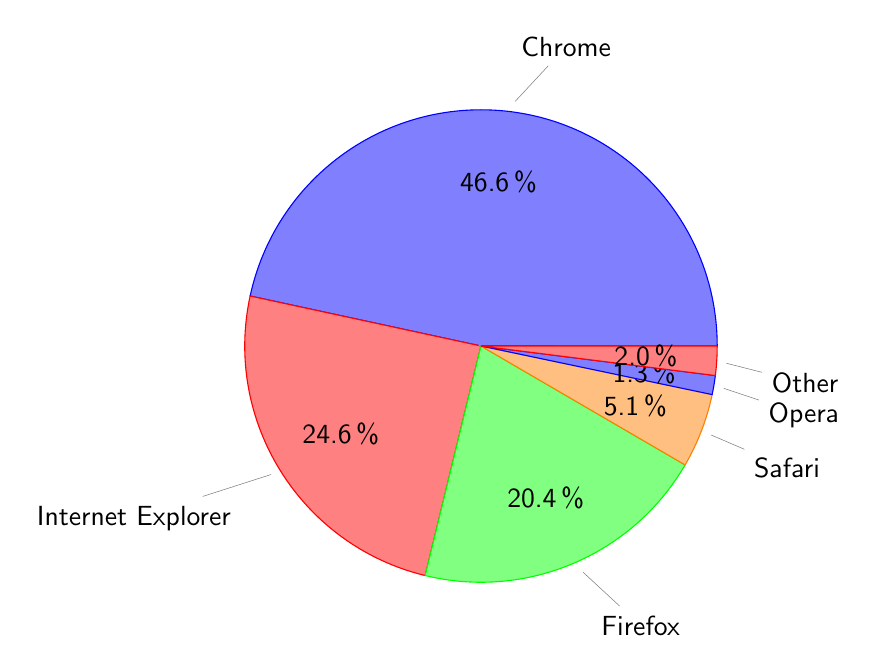
\begin{tikzpicture}[nodes = {font=\sffamily}]
  \foreach \percent/\name in {
      46.6/Chrome,
      24.6/Internet Explorer,
      20.4/Firefox,
      5.1/Safari,
      1.3/Opera,
      2.0/Other
    } {
      \ifx\percent\empty\else               % If \percent is empty, do nothing
        \global\advance\cyclecount by 1     % Advance cyclecount
        \global\advance\ind by 1            % Advance list index
        \ifnum3<\cyclecount                 % If cyclecount is larger than list
          \global\cyclecount=0              %   reset cyclecount and
          \global\ind=0                     %   reset list index
        \fi
        \pgfmathparse{\cyclelist[\the\ind]} % Get color from cycle list
        \edef\color{\pgfmathresult}         %   and store as \color
        % Draw angle and set labels
        \draw[fill={\color!50},draw={\color}] (0,0) -- (\angle:\radius)
          arc (\angle:\angle+\percent*3.6:\radius) -- cycle;
        \node at (\angle+0.5*\percent*3.6:0.7*\radius) {\percent\,\%};
        \node[pin=\angle+0.5*\percent*3.6:\name]
          at (\angle+0.5*\percent*3.6:\radius) {};
        \pgfmathparse{\angle+\percent*3.6}  % Advance angle
        \xdef\angle{\pgfmathresult}         %   and store in \angle
      \fi
    };
\end{tikzpicture}


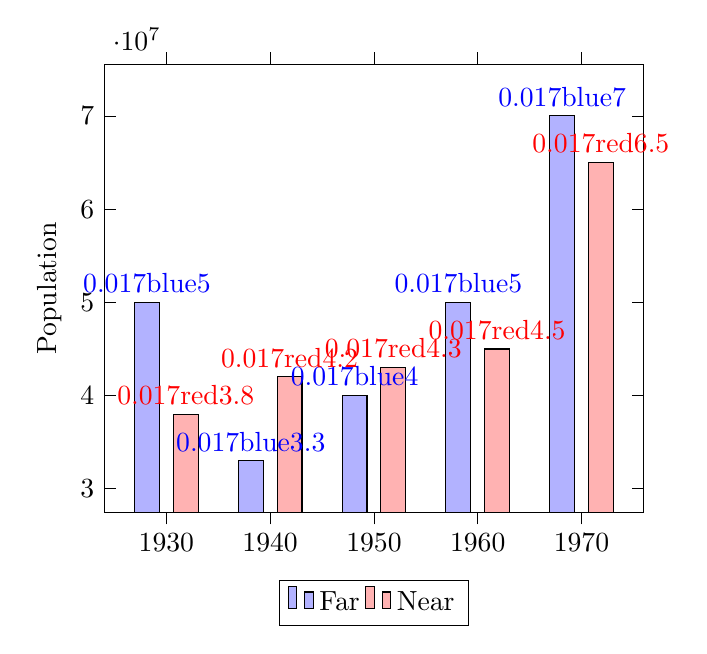
\begin{tikzpicture} 
\begin{axis}[ 
			x tick label style={ /pgf/number format/1000 sep=}, 
			ylabel=Population, enlargelimits=0.15, 
			legend style={at={(0.5,-0.15)}, 
			anchor=north,legend columns=-1}, 
			ybar=5pt,% configures `bar shift' 
			bar width=9pt, nodes near coords, point meta=y *10^-7 % the displayed number 
] 
\addplot 
	coordinates {(1930,50e6) (1940,33e6) (1950,40e6) (1960,50e6) (1970,70e6)}; 
\addplot 
	coordinates {(1930,38e6) (1940,42e6) (1950,43e6) (1960,45e6) (1970,65e6)}; 
\legend{Far,Near} 
\end{axis} 
\end{tikzpicture}